\section{Constant Volatility}
This chapter will delve into the limitations 
of the Black-Scholes model, particularly its 
assumption of constant volatility, and introduce 
the SABR model as a more dynamic alternative for estimating volatility. 
The chapter will illustrate the inconsistency of 
this assumption with real-world market data, 
using the S$\&$P 500 index and the 10Y10Y EUR swaption 
as examples.
\\\\
The Black-Scholes model, introduced earlier, outlines the pricing formula for a European call option in 
Proposition \autoref{Black-Scholes Formula}. It is  essential to recall that in the Black-Scholes formula, 
volatility is considered constant. This implies that the volatility of the asset's returns does not vary over time,
establishing a direct correlation between the option's price and its volatility. Consequently, 
understanding implied volatility becomes crucial. Although the Black Scholes model does not provide 
a closed-form solution for implied volatility, it can be determined numerically, a topic not covered 
in this analysis. Instead, we introduce the SABR model to estimate volatility, which can then be 
applied to the Black Scholes model for option pricing. This will be covered in the Section about the 
SABR model. 
\\\\
We will briefly demonstrate why the assumption of constant volatility is inconsistent with market data. 
Our analysis includes an examination of the S$\&$P 500 index and the 10Y10Y EUR swaption, which are frequently used 
financial indicators. 
\\\\
As depicted in \autoref{10Y10Y dev} and \autoref{sp500 dev}, the development of the 10Y10Y EUR swaption 
and S$\&$P 500 index levels illustrates fluctuations over time. This variability is further emphasized by the return patterns 
shown in \autoref{10Y10Y return} and \autoref{sp500 return}, where the returns of the 10Y10Y EUR swaption and S$\&$P 500 index are plotted. 
These fluctuations suggest that market volatility is not constant. Our analysis underscores that volatility varies 
significantly from day to day, reflecting the market's response to new information and events. This observation challenges 
the applicability of the Black-Scholes model, which assumes constant volatility and highlights the need for models like the 
SABR model that more accurately capture market dynamics and provide nuanced volatility estimates.
\begin{figure}[h]
    \centering
    \begin{minipage}{0.5\textwidth}
        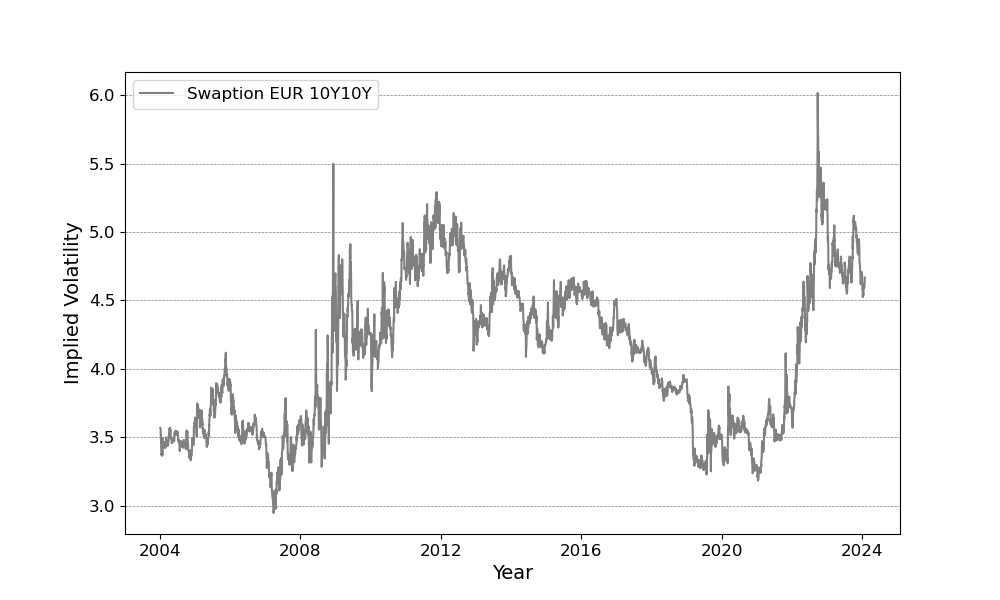
\includegraphics[width=\linewidth]{/Users/nannaingemannohrt/Desktop/master_thesis/main/plots/10Y10Yswaption.png}
        \caption{Swaption EUR 10Y10Y from  2004-01-01 \\ to 2024-01-01.}
        \label{10Y10Y dev}
    \end{minipage}\hfill 
    \begin{minipage}{0.5\textwidth}
        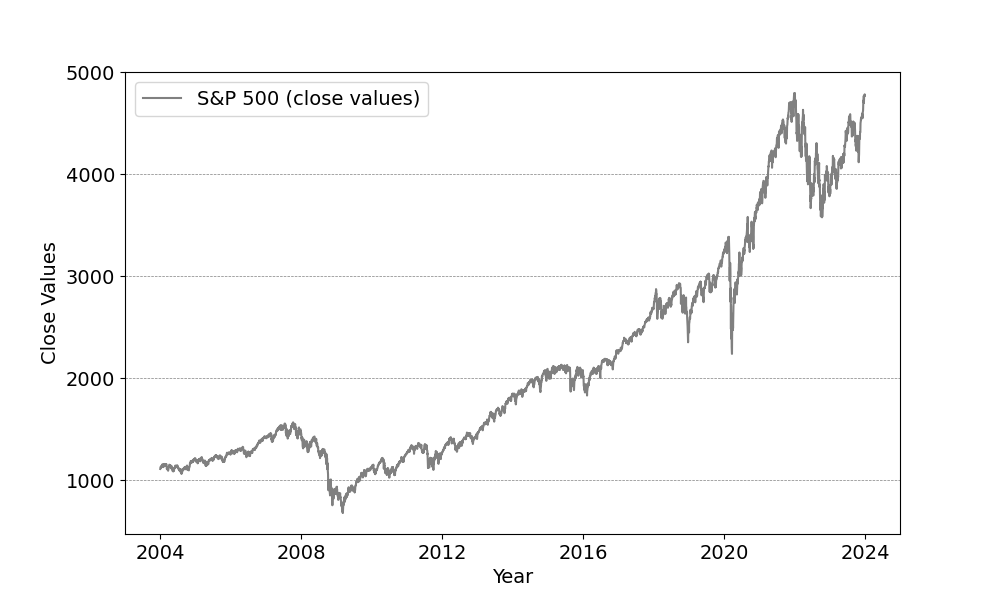
\includegraphics[width=\linewidth]{/Users/nannaingemannohrt/Desktop/master_thesis/main/plots/sp500.png}
        \caption{S$\&$P500 index (close values) from \\ 2004-01-01 to 2024-01-01.}
        \label{sp500 dev}
    \end{minipage}
\end{figure}
\newpage
\begin{figure}[h]
    \centering
    \begin{minipage}{0.5\textwidth}
        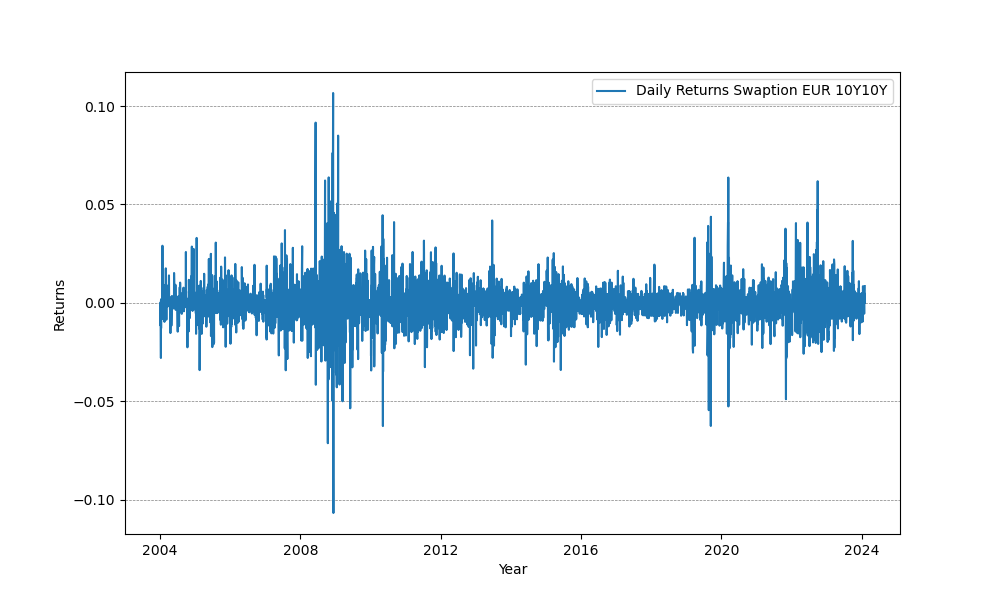
\includegraphics[width=\linewidth]{/Users/nannaingemannohrt/Desktop/master_thesis/main/plots/10Y10Yswaptionreturn.png}
        \caption{Swaption EUR 10Y10Y return from  \\ 2004-01-01 to 2024-01-01.}
        \label{10Y10Y return}
    \end{minipage}\hfill 
    \begin{minipage}{0.5\textwidth}
        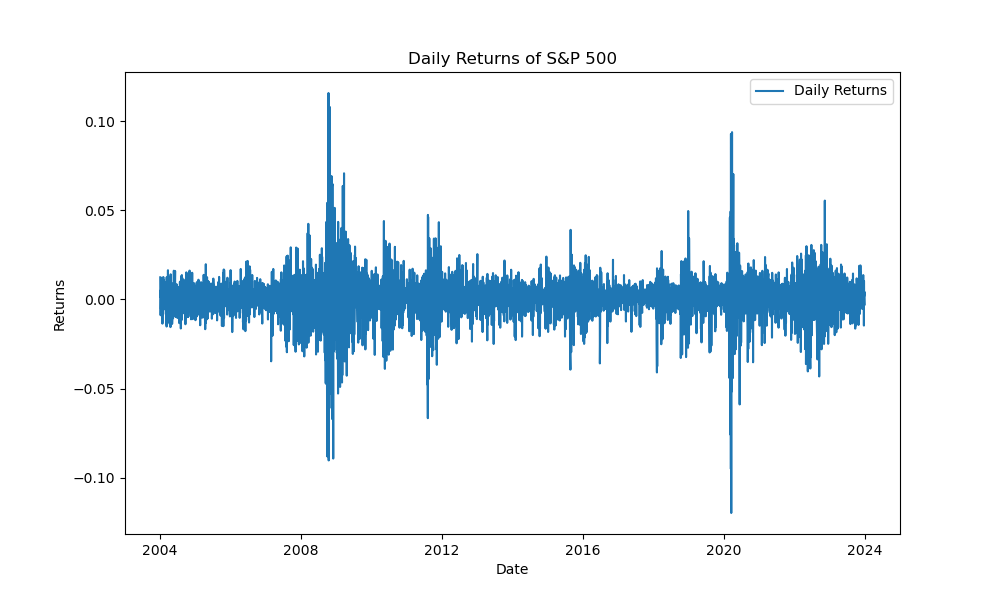
\includegraphics[width=\linewidth]{/Users/nannaingemannohrt/Desktop/master_thesis/main/plots/sp500return.png}
        \caption{S$\&$P500 index (close values) return  \\ from 2004-01-01 to 2024-01-01.}
        \label{sp500 return}
    \end{minipage}
\end{figure}
\noindent
\\\\
A brief review of the market data reveals a trend in 
volatility, indicating that it is not constant. 
Given this fluctuation, how should we proceed when 
considering to be able to price a swaption? We will continue our 
analysis by exploring a two-factor model rather 
than the previously described one-factor Vasicek model. 
This approach allows us to model volatility 
stochastically and use the resulting volatility 
estimates to price a swaption in the Black Scholes model. 
